\section{Implementation of the Safety Annex}
\label{sec:impl}
The Safety Annex is written in Java as a plug-in for the OSATE AADL toolset, which is built on Eclipse.  It is not designed as a stand-alone extension of the language, but works with behavioral contracts specified using the AGREE annex for AADL~\cite{NFM2012:CoGaMiWhLaLu}. 
The architecture of the Safety Annex is shown in Figure~\ref{fig:plugin-arch}.

\begin{figure}[h]
	\begin{center}
		%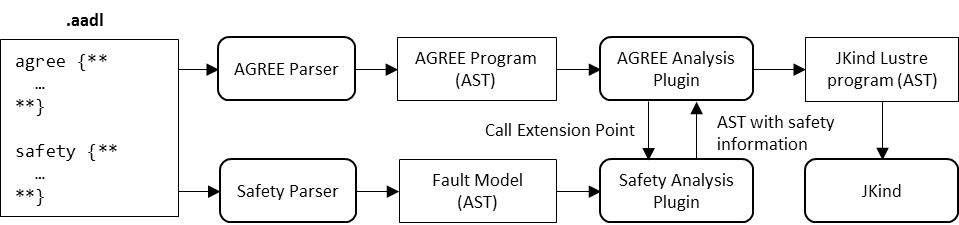
\includegraphics[trim=0 400 430 0,clip,width=0.85\textwidth]{images/arch.png}
		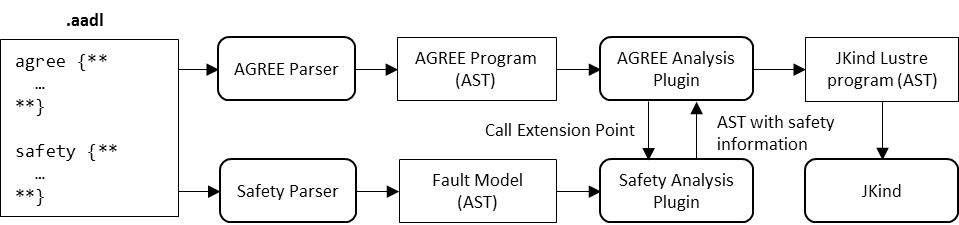
\includegraphics[width=\textwidth]{images/arch.png}
	\end{center}
	%\vspace{-0.2in}
	\caption{Safety Annex Plug-in Architecture}
	\label{fig:plugin-arch}
	%\vspace{-0.2in}
\end{figure}

AGREE contracts are used to define the nominal behaviors of system components as {\em guarantees} that hold when {\em assumptions} about the values the component's environment are met. When an AADL model is annotated with AGREE contracts and the fault model is created using the Safety Annex, the model is transformed through AGREE into a Lustre model~\cite{Halbwachs91:IEEE} containing the behavioral extensions defined in the AGREE contracts for each system component. 

When performing fault analysis, the Safety Annex extends the AGREE contracts to allow faults to modify the behavior of component inputs and outputs. An example of a portion of an initial AGREE node and its extended contract is shown in Figure~\ref{fig:lustre}. The left column of the figure shows the nominal Lustre pump definition is shown with an AGREE contract on the output; and the right column shows the additional local variables for the fault (boxes 1 and 2), the assertion binding the fault value to the nominal value (boxes 3 and 4), and the fault node definition (box 5). Once augmented with fault information, the AGREE model (translated into the Lustre dataflow language~\cite{Halbwachs91:IEEE}) follows the standard translation path to the model checker JKind~\cite{2017arXiv171201222G}, an infinite-state model checker for safety properties. 

\begin{figure}[h!]
	%\hspace*{-2cm}
	%\vspace{-0.3in} 
	\begin{center}
		%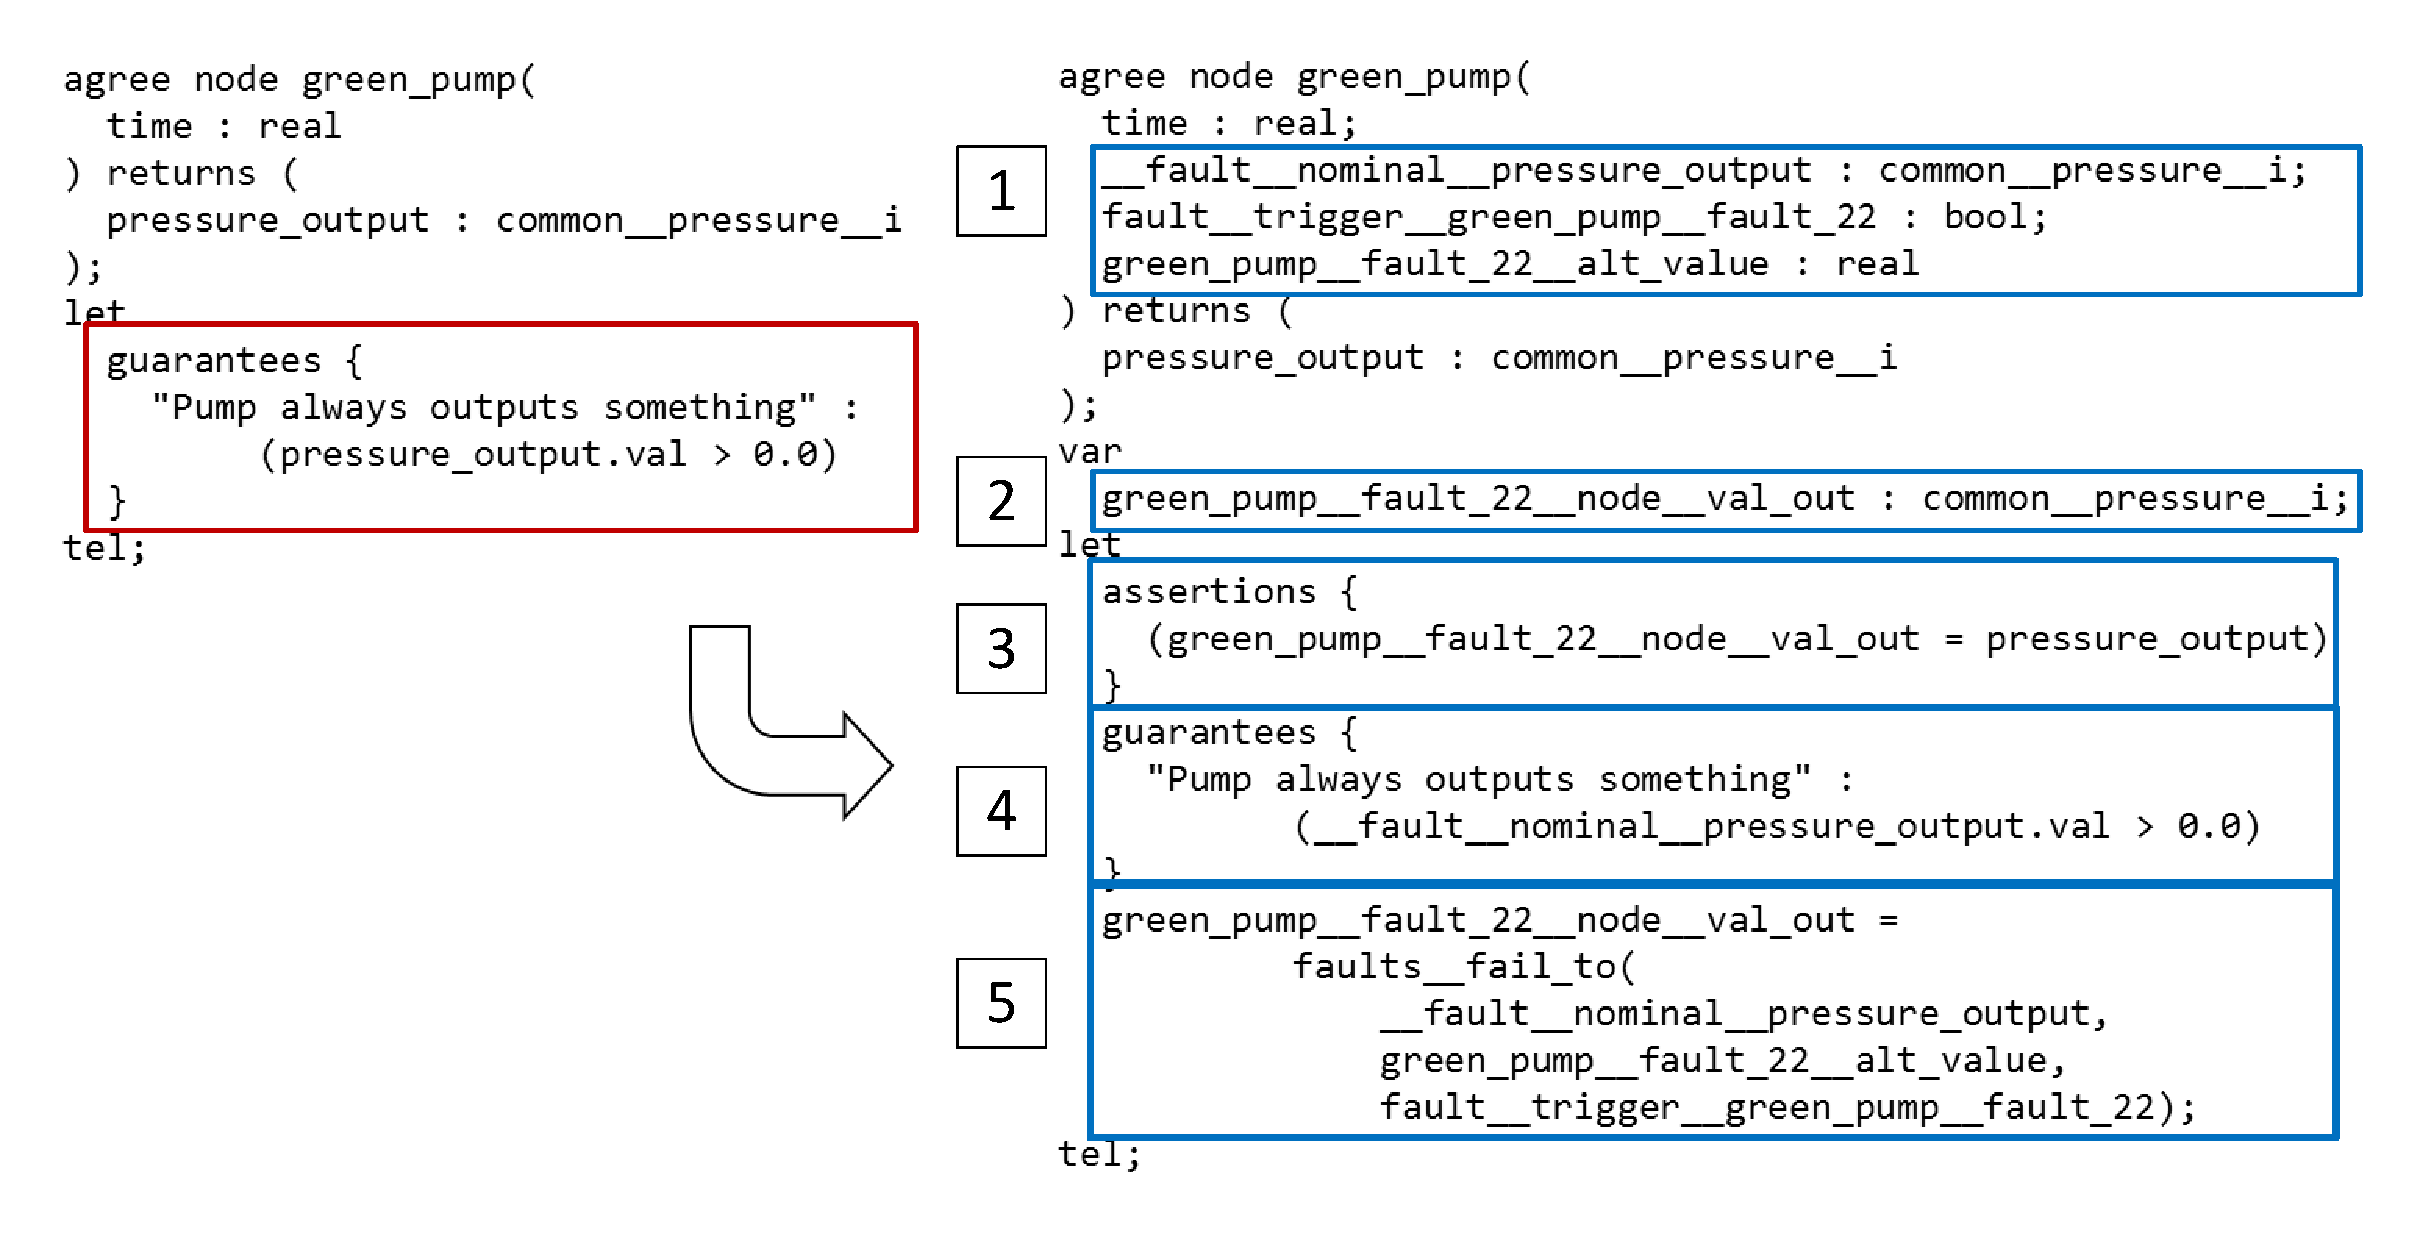
\includegraphics[trim=0 690 -10 70,clip,width=1.5\dimexpr\textwidth-2cm\relax]{images/lustre.pdf}
		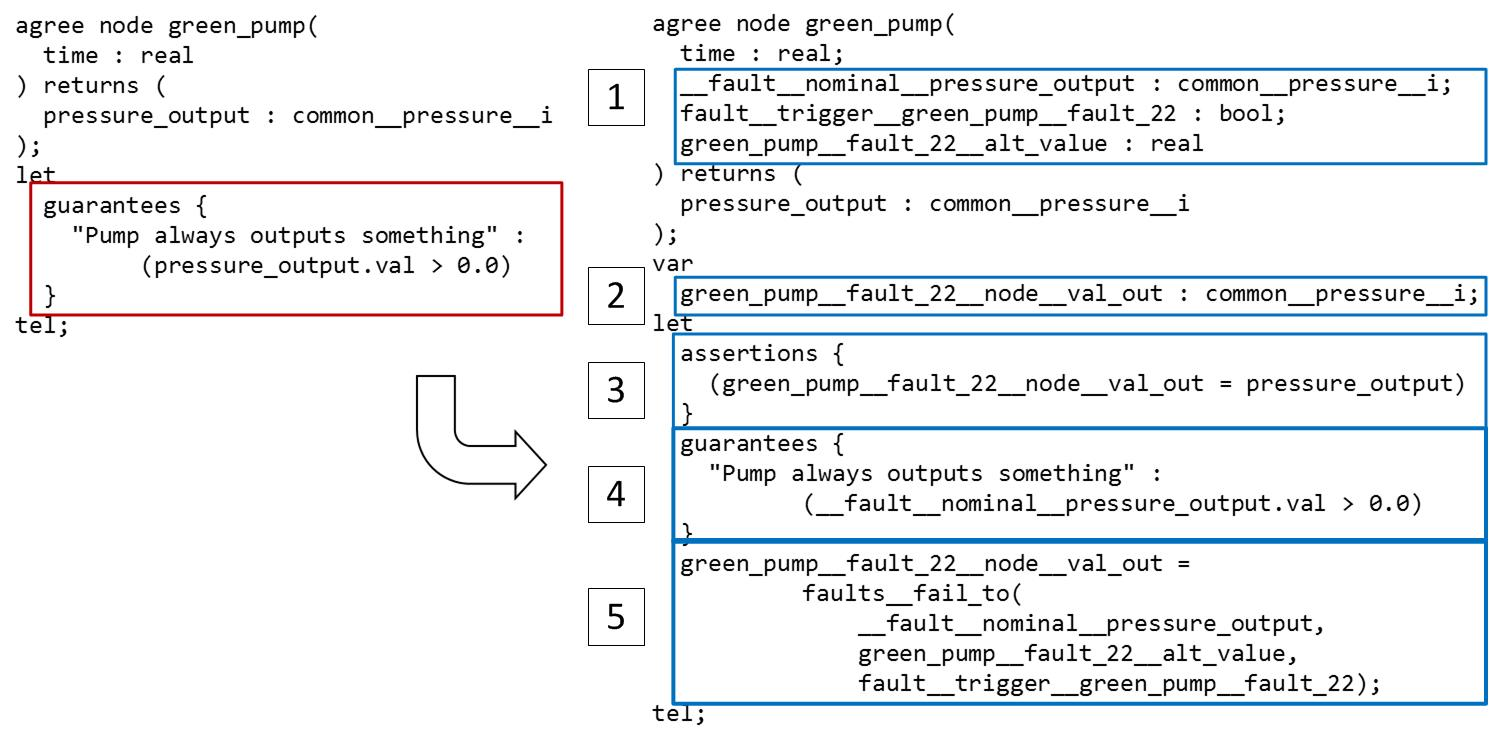
\includegraphics[scale=0.3]{images/lustre.jpg}
		%\caption{Nominal AGREE node and its extension with faults}
		\caption{Nominal AGREE Node and Extension with Faults}
		\label{fig:lustre}
	\end{center}
	%\vspace{-0.3in}
\end{figure}

There are two different types of fault analysis that can be performed on a fault model. The Safety Annex plugin intercepts the AGREE program and add fault model information to the model depending on which form of fault analysis is being run.

\textbf{Verification in the Presence of Faults}: This analysis returns one counterexample when fault activation per the fault hypothesis can cause violation of a property. The augmentation from Safety Annex to the AGREE program includes traceability information so that when counterexamples are displayed to users, the active faults for each component are visualized.

\textbf{Generate Minimal Cut Sets}: This analysis collects all minimal set of fault combinations that can cause violation of a property. As described in Chapter~\ref{chap:mcsGen}, the first step of MinCutSet generation is to collect the minimal IVCs for each property. Given the compositional nature of the verification, each level of the system is extended in a slightly different way. The leaf nodes of a system contribute only constrained faults to the \aivcalg algorithm as shown in Figure~\ref{fig:ivcElements1}. 

\begin{figure}[h!]
	\hspace*{-2cm}
	\vspace{-0.1in} 
	\begin{center}
		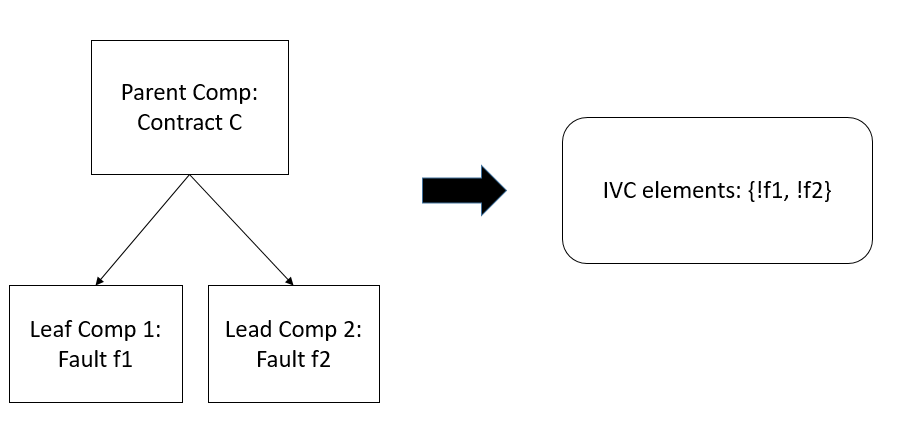
\includegraphics[scale=0.5]{images/ivcElements1.png}
	\caption{IVC Elements used for Consideration in a Leaf Layer of a System}
		\label{fig:ivcElements1}
	\end{center}
\end{figure}

In the non-leaf layers of the program, both contracts and constrained faults are considered as shown in Figure~\ref{fig:ivcElements2}. The reason for this is that the contracts are used to prove the properties at the next highest level and are necessary for the verification of the properties. 

\begin{figure}[h!]
	\hspace*{-2cm}
	\vspace{-0.1in} 
	\begin{center}
		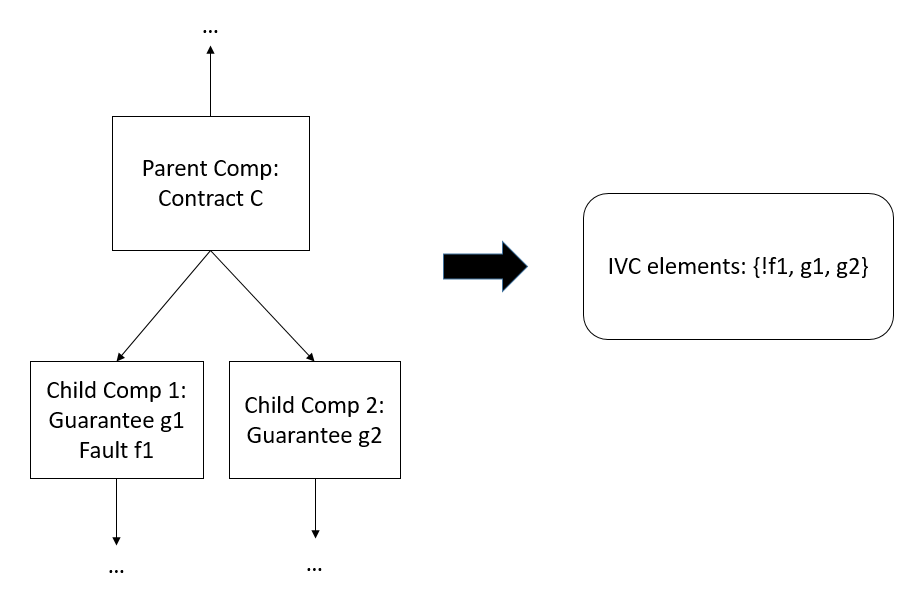
\includegraphics[scale=0.5]{images/ivcElements2.png}
	\caption{IVC Elements used for Consideration in a Middle Layer of a System}
		\label{fig:ivcElements2}
	\end{center}
\end{figure}

The \aivcalg algorithm returns the minimal set of these elements necessary to prove the properties. This equates to any contracts or inactive faults that must be present in order for the verification of properties in the model. From here, we transform all MIVCs into minimal cut sets.

